% Graphic for TeX using PGF
% Title: /home/andre/GIT Repos/AHCampher_thesis/diagrams/sampleaisaos.dia
% Creator: Dia v0.97.1
% CreationDate: Thu Jan  6 14:07:33 2011
% For: andre
% \usepackage{tikz}
% The following commands are not supported in PSTricks at present
% We define them conditionally, so when they are implemented,
% this pgf file will use them.
\ifx\du\undefined
  \newlength{\du}
\fi
\setlength{\du}{15\unitlength}
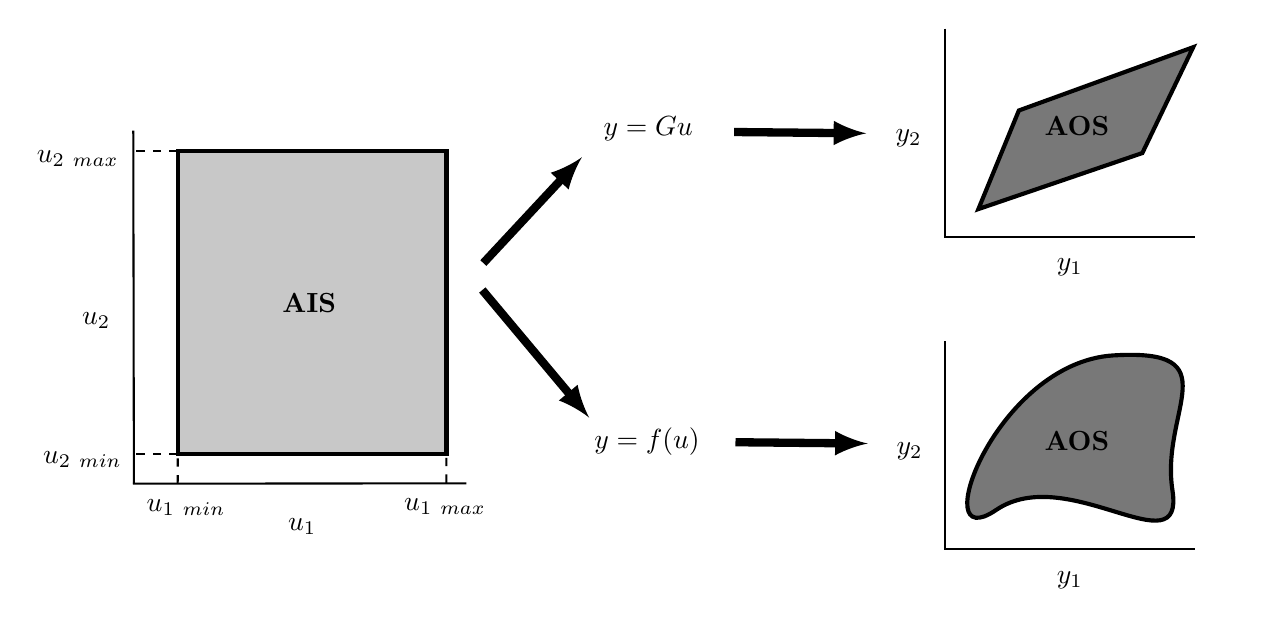
\begin{tikzpicture}
\pgftransformxscale{1.000000}
\pgftransformyscale{-1.000000}
\definecolor{dialinecolor}{rgb}{0.000000, 0.000000, 0.000000}
\pgfsetstrokecolor{dialinecolor}
\definecolor{dialinecolor}{rgb}{1.000000, 1.000000, 1.000000}
\pgfsetfillcolor{dialinecolor}
\pgfsetlinewidth{0.100000\du}
\pgfsetdash{}{0pt}
\pgfsetdash{}{0pt}
\pgfsetmiterjoin
\definecolor{dialinecolor}{rgb}{0.784314, 0.784314, 0.784314}
\pgfsetfillcolor{dialinecolor}
\fill (1.574384\du,2.981260\du)--(1.574384\du,10.281260\du)--(8.047075\du,10.281260\du)--(8.047075\du,2.981260\du)--cycle;
\definecolor{dialinecolor}{rgb}{0.000000, 0.000000, 0.000000}
\pgfsetstrokecolor{dialinecolor}
\draw (1.574384\du,2.981260\du)--(1.574384\du,10.281260\du)--(8.047075\du,10.281260\du)--(8.047075\du,2.981260\du)--cycle;
\pgfsetlinewidth{0.050000\du}
\pgfsetdash{}{0pt}
\pgfsetdash{}{0pt}
\pgfsetbuttcap
{
\definecolor{dialinecolor}{rgb}{0.000000, 0.000000, 0.000000}
\pgfsetfillcolor{dialinecolor}
% was here!!!
\definecolor{dialinecolor}{rgb}{0.000000, 0.000000, 0.000000}
\pgfsetstrokecolor{dialinecolor}
\draw (0.503325\du,2.493750\du)--(0.518134\du,10.993760\du);
}
\pgfsetlinewidth{0.050000\du}
\pgfsetdash{}{0pt}
\pgfsetdash{}{0pt}
\pgfsetbuttcap
{
\definecolor{dialinecolor}{rgb}{0.000000, 0.000000, 0.000000}
\pgfsetfillcolor{dialinecolor}
% was here!!!
\definecolor{dialinecolor}{rgb}{0.000000, 0.000000, 0.000000}
\pgfsetstrokecolor{dialinecolor}
\draw (8.525166\du,10.989073\du)--(0.492855\du,10.995323\du);
}
\pgfsetlinewidth{0.050000\du}
\pgfsetdash{{1.000000\du}{1.000000\du}}{0\du}
\pgfsetdash{{0.200000\du}{0.200000\du}}{0\du}
\pgfsetbuttcap
{
\definecolor{dialinecolor}{rgb}{0.000000, 0.000000, 0.000000}
\pgfsetfillcolor{dialinecolor}
% was here!!!
\definecolor{dialinecolor}{rgb}{0.000000, 0.000000, 0.000000}
\pgfsetstrokecolor{dialinecolor}
\draw (1.573559\du,10.987510\du)--(1.574384\du,10.281260\du);
}
\pgfsetlinewidth{0.050000\du}
\pgfsetdash{{0.200000\du}{0.200000\du}}{0\du}
\pgfsetdash{{0.200000\du}{0.200000\du}}{0\du}
\pgfsetbuttcap
{
\definecolor{dialinecolor}{rgb}{0.000000, 0.000000, 0.000000}
\pgfsetfillcolor{dialinecolor}
% was here!!!
\definecolor{dialinecolor}{rgb}{0.000000, 0.000000, 0.000000}
\pgfsetstrokecolor{dialinecolor}
\draw (8.047594\du,10.975010\du)--(8.047075\du,10.281260\du);
}
\pgfsetlinewidth{0.050000\du}
\pgfsetdash{{0.200000\du}{0.200000\du}}{0\du}
\pgfsetdash{{0.200000\du}{0.200000\du}}{0\du}
\pgfsetbuttcap
{
\definecolor{dialinecolor}{rgb}{0.000000, 0.000000, 0.000000}
\pgfsetfillcolor{dialinecolor}
% was here!!!
\definecolor{dialinecolor}{rgb}{0.000000, 0.000000, 0.000000}
\pgfsetstrokecolor{dialinecolor}
\draw (1.574384\du,10.281260\du)--(0.526684\du,10.281260\du);
}
\pgfsetlinewidth{0.050000\du}
\pgfsetdash{{0.200000\du}{0.200000\du}}{0\du}
\pgfsetdash{{0.200000\du}{0.200000\du}}{0\du}
\pgfsetbuttcap
{
\definecolor{dialinecolor}{rgb}{0.000000, 0.000000, 0.000000}
\pgfsetfillcolor{dialinecolor}
% was here!!!
\definecolor{dialinecolor}{rgb}{0.000000, 0.000000, 0.000000}
\pgfsetstrokecolor{dialinecolor}
\draw (1.574384\du,2.981260\du)--(0.519417\du,2.981260\du);
}
% setfont left to latex
\definecolor{dialinecolor}{rgb}{0.000000, 0.000000, 0.000000}
\pgfsetstrokecolor{dialinecolor}
\node[anchor=west] at (-0.978316\du,7.075781\du){$u_2$};
% setfont left to latex
\definecolor{dialinecolor}{rgb}{0.000000, 0.000000, 0.000000}
\pgfsetstrokecolor{dialinecolor}
\node[anchor=west] at (3.984184\du,12.025781\du){$u_1$};
% setfont left to latex
\definecolor{dialinecolor}{rgb}{0.000000, 0.000000, 0.000000}
\pgfsetstrokecolor{dialinecolor}
\node[anchor=west] at (-2.065816\du,3.163281\du){$u_{2~max}$};
% setfont left to latex
\definecolor{dialinecolor}{rgb}{0.000000, 0.000000, 0.000000}
\pgfsetstrokecolor{dialinecolor}
\node[anchor=west] at (-1.917066\du,10.410781\du){$u_{2~min}$};
% setfont left to latex
\definecolor{dialinecolor}{rgb}{0.000000, 0.000000, 0.000000}
\pgfsetstrokecolor{dialinecolor}
\node[anchor=west] at (6.781684\du,11.550791\du){$u_{1~max}$};
% setfont left to latex
\definecolor{dialinecolor}{rgb}{0.000000, 0.000000, 0.000000}
\pgfsetstrokecolor{dialinecolor}
\node[anchor=west] at (0.580434\du,11.565791\du){$u_{1~min}$};
\pgfsetlinewidth{0.050000\du}
\pgfsetdash{}{0pt}
\pgfsetdash{}{0pt}
\pgfsetbuttcap
{
\definecolor{dialinecolor}{rgb}{0.000000, 0.000000, 0.000000}
\pgfsetfillcolor{dialinecolor}
% was here!!!
\definecolor{dialinecolor}{rgb}{0.000000, 0.000000, 0.000000}
\pgfsetstrokecolor{dialinecolor}
\draw (20.050825\du,0.036250\du)--(20.050825\du,5.061250\du);
}
\pgfsetlinewidth{0.050000\du}
\pgfsetdash{}{0pt}
\pgfsetdash{}{0pt}
\pgfsetbuttcap
{
\definecolor{dialinecolor}{rgb}{0.000000, 0.000000, 0.000000}
\pgfsetfillcolor{dialinecolor}
% was here!!!
\definecolor{dialinecolor}{rgb}{0.000000, 0.000000, 0.000000}
\pgfsetstrokecolor{dialinecolor}
\draw (26.075825\du,5.048750\du)--(20.025825\du,5.048750\du);
}
% setfont left to latex
\definecolor{dialinecolor}{rgb}{0.000000, 0.000000, 0.000000}
\pgfsetstrokecolor{dialinecolor}
\node[anchor=west] at (18.619184\du,2.680781\du){$y_2$};
% setfont left to latex
\definecolor{dialinecolor}{rgb}{0.000000, 0.000000, 0.000000}
\pgfsetstrokecolor{dialinecolor}
\node[anchor=west] at (22.506684\du,5.780781\du){$y_1$};
\pgfsetlinewidth{0.050000\du}
\pgfsetdash{}{0pt}
\pgfsetdash{}{0pt}
\pgfsetbuttcap
{
\definecolor{dialinecolor}{rgb}{0.000000, 0.000000, 0.000000}
\pgfsetfillcolor{dialinecolor}
% was here!!!
\definecolor{dialinecolor}{rgb}{0.000000, 0.000000, 0.000000}
\pgfsetstrokecolor{dialinecolor}
\draw (20.050925\du,7.566260\du)--(20.050925\du,12.591260\du);
}
\pgfsetlinewidth{0.050000\du}
\pgfsetdash{}{0pt}
\pgfsetdash{}{0pt}
\pgfsetbuttcap
{
\definecolor{dialinecolor}{rgb}{0.000000, 0.000000, 0.000000}
\pgfsetfillcolor{dialinecolor}
% was here!!!
\definecolor{dialinecolor}{rgb}{0.000000, 0.000000, 0.000000}
\pgfsetstrokecolor{dialinecolor}
\draw (26.075925\du,12.578760\du)--(20.025925\du,12.578760\du);
}
% setfont left to latex
\definecolor{dialinecolor}{rgb}{0.000000, 0.000000, 0.000000}
\pgfsetstrokecolor{dialinecolor}
\node[anchor=west] at (18.644284\du,10.210791\du){$y_2$};
% setfont left to latex
\definecolor{dialinecolor}{rgb}{0.000000, 0.000000, 0.000000}
\pgfsetstrokecolor{dialinecolor}
\node[anchor=west] at (22.506784\du,13.310791\du){$y_1$};
\pgfsetlinewidth{0.100000\du}
\pgfsetdash{}{0pt}
\pgfsetdash{}{0pt}
\pgfsetmiterjoin
\pgfsetbuttcap
\definecolor{dialinecolor}{rgb}{0.470588, 0.470588, 0.470588}
\pgfsetfillcolor{dialinecolor}
\fill (21.836784\du,2.006260\du)--(20.861784\du,4.381260\du)--(24.811784\du,3.031260\du)--(26.036784\du,0.481260\du)--cycle;
\definecolor{dialinecolor}{rgb}{0.000000, 0.000000, 0.000000}
\pgfsetstrokecolor{dialinecolor}
\draw (21.836784\du,2.006260\du)--(20.861784\du,4.381260\du)--(24.811784\du,3.031260\du)--(26.036784\du,0.481260\du)--cycle;
\pgfsetlinewidth{0.100000\du}
\pgfsetdash{}{0pt}
\pgfsetdash{}{0pt}
\pgfsetmiterjoin
\pgfsetbuttcap
\definecolor{dialinecolor}{rgb}{0.470588, 0.470588, 0.470588}
\pgfsetfillcolor{dialinecolor}
\pgfpathmoveto{\pgfpoint{21.286784\du}{11.631260\du}}
\pgfpathcurveto{\pgfpoint{23.011784\du}{10.456260\du}}{\pgfpoint{25.836784\du}{13.081260\du}}{\pgfpoint{25.536784\du}{11.156260\du}}
\pgfpathcurveto{\pgfpoint{25.236784\du}{9.231260\du}}{\pgfpoint{26.961784\du}{7.731260\du}}{\pgfpoint{24.111784\du}{7.906260\du}}
\pgfpathcurveto{\pgfpoint{21.261784\du}{8.081260\du}}{\pgfpoint{19.561784\du}{12.806260\du}}{\pgfpoint{21.286784\du}{11.631260\du}}
\pgfusepath{fill}
\definecolor{dialinecolor}{rgb}{0.000000, 0.000000, 0.000000}
\pgfsetstrokecolor{dialinecolor}
\pgfpathmoveto{\pgfpoint{21.286784\du}{11.631260\du}}
\pgfpathcurveto{\pgfpoint{23.011784\du}{10.456260\du}}{\pgfpoint{25.836784\du}{13.081260\du}}{\pgfpoint{25.536784\du}{11.156260\du}}
\pgfpathcurveto{\pgfpoint{25.236784\du}{9.231260\du}}{\pgfpoint{26.961784\du}{7.731260\du}}{\pgfpoint{24.111784\du}{7.906260\du}}
\pgfpathcurveto{\pgfpoint{21.261784\du}{8.081260\du}}{\pgfpoint{19.561784\du}{12.806260\du}}{\pgfpoint{21.286784\du}{11.631260\du}}
\pgfusepath{stroke}
% setfont left to latex
\definecolor{dialinecolor}{rgb}{0.000000, 0.000000, 0.000000}
\pgfsetstrokecolor{dialinecolor}
\node[anchor=west] at (11.561784\du,2.456260\du){$y = G\vect{u}$};
% setfont left to latex
\definecolor{dialinecolor}{rgb}{0.000000, 0.000000, 0.000000}
\pgfsetstrokecolor{dialinecolor}
\node[anchor=west] at (11.336784\du,9.981260\du){$y = f(\vect{u})$};
\pgfsetlinewidth{0.200000\du}
\pgfsetdash{}{0pt}
\pgfsetdash{}{0pt}
\pgfsetbuttcap
{
\definecolor{dialinecolor}{rgb}{0.000000, 0.000000, 0.000000}
\pgfsetfillcolor{dialinecolor}
% was here!!!
\pgfsetarrowsend{latex}
\definecolor{dialinecolor}{rgb}{0.000000, 0.000000, 0.000000}
\pgfsetstrokecolor{dialinecolor}
\draw (8.936884\du,5.681260\du)--(11.311884\du,3.131260\du);
}
\pgfsetlinewidth{0.200000\du}
\pgfsetdash{}{0pt}
\pgfsetdash{}{0pt}
\pgfsetbuttcap
{
\definecolor{dialinecolor}{rgb}{0.000000, 0.000000, 0.000000}
\pgfsetfillcolor{dialinecolor}
% was here!!!
\pgfsetarrowsend{latex}
\definecolor{dialinecolor}{rgb}{0.000000, 0.000000, 0.000000}
\pgfsetstrokecolor{dialinecolor}
\draw (8.911884\du,6.331260\du)--(11.486884\du,9.406260\du);
}
\pgfsetlinewidth{0.200000\du}
\pgfsetdash{}{0pt}
\pgfsetdash{}{0pt}
\pgfsetbuttcap
{
\definecolor{dialinecolor}{rgb}{0.000000, 0.000000, 0.000000}
\pgfsetfillcolor{dialinecolor}
% was here!!!
\pgfsetarrowsend{latex}
\definecolor{dialinecolor}{rgb}{0.000000, 0.000000, 0.000000}
\pgfsetstrokecolor{dialinecolor}
\draw (14.975717\du,2.524889\du)--(18.161884\du,2.556260\du);
}
\pgfsetlinewidth{0.200000\du}
\pgfsetdash{}{0pt}
\pgfsetdash{}{0pt}
\pgfsetbuttcap
{
\definecolor{dialinecolor}{rgb}{0.000000, 0.000000, 0.000000}
\pgfsetfillcolor{dialinecolor}
% was here!!!
\pgfsetarrowsend{latex}
\definecolor{dialinecolor}{rgb}{0.000000, 0.000000, 0.000000}
\pgfsetstrokecolor{dialinecolor}
\draw (15.010364\du,9.997580\du)--(18.196532\du,10.028951\du);
}
\node at (2.5,3.5){{\bf AIS}};
\node at (12.25,1.25){{\bf AOS}};
\node at (12.25,5.25){{\bf AOS}};
\end{tikzpicture}
